%\clearpage

\subsection{NMF Synchronizations}
\label{sec:NMF}

\NOTE{\emph{Solution expert:} Georg, \emph{Interviewer:} Bernhard}

\subsubsection{Approach}
\label{sec:ApproachNMF}

NMF Synchronizations \cite{SoSyM2017-Hinkel}is a bx language which is formally based on category theory. Consistency between two models is defined in terms of consistency relations between their elements. In the case of mutual consistency, an element-level consistency relation is an \emph{isomorphism} between typed source and target elements, i.e., a bijective mapping between elements of some type $A$ in the source model and elements of some type $C$ in the target model satisfying specified consistency constraints. Consistency relations are coupled: For an $A$-element to be consistent with a $C$-element, an isomorphism between dependent source and target elements (of types $B$ and $D$)may be required. In addition to defining element-level consistency relations, consistency restoration has to be specified, provided that no default restoration is available.

\begin{figure}[tb!]
	\centering
	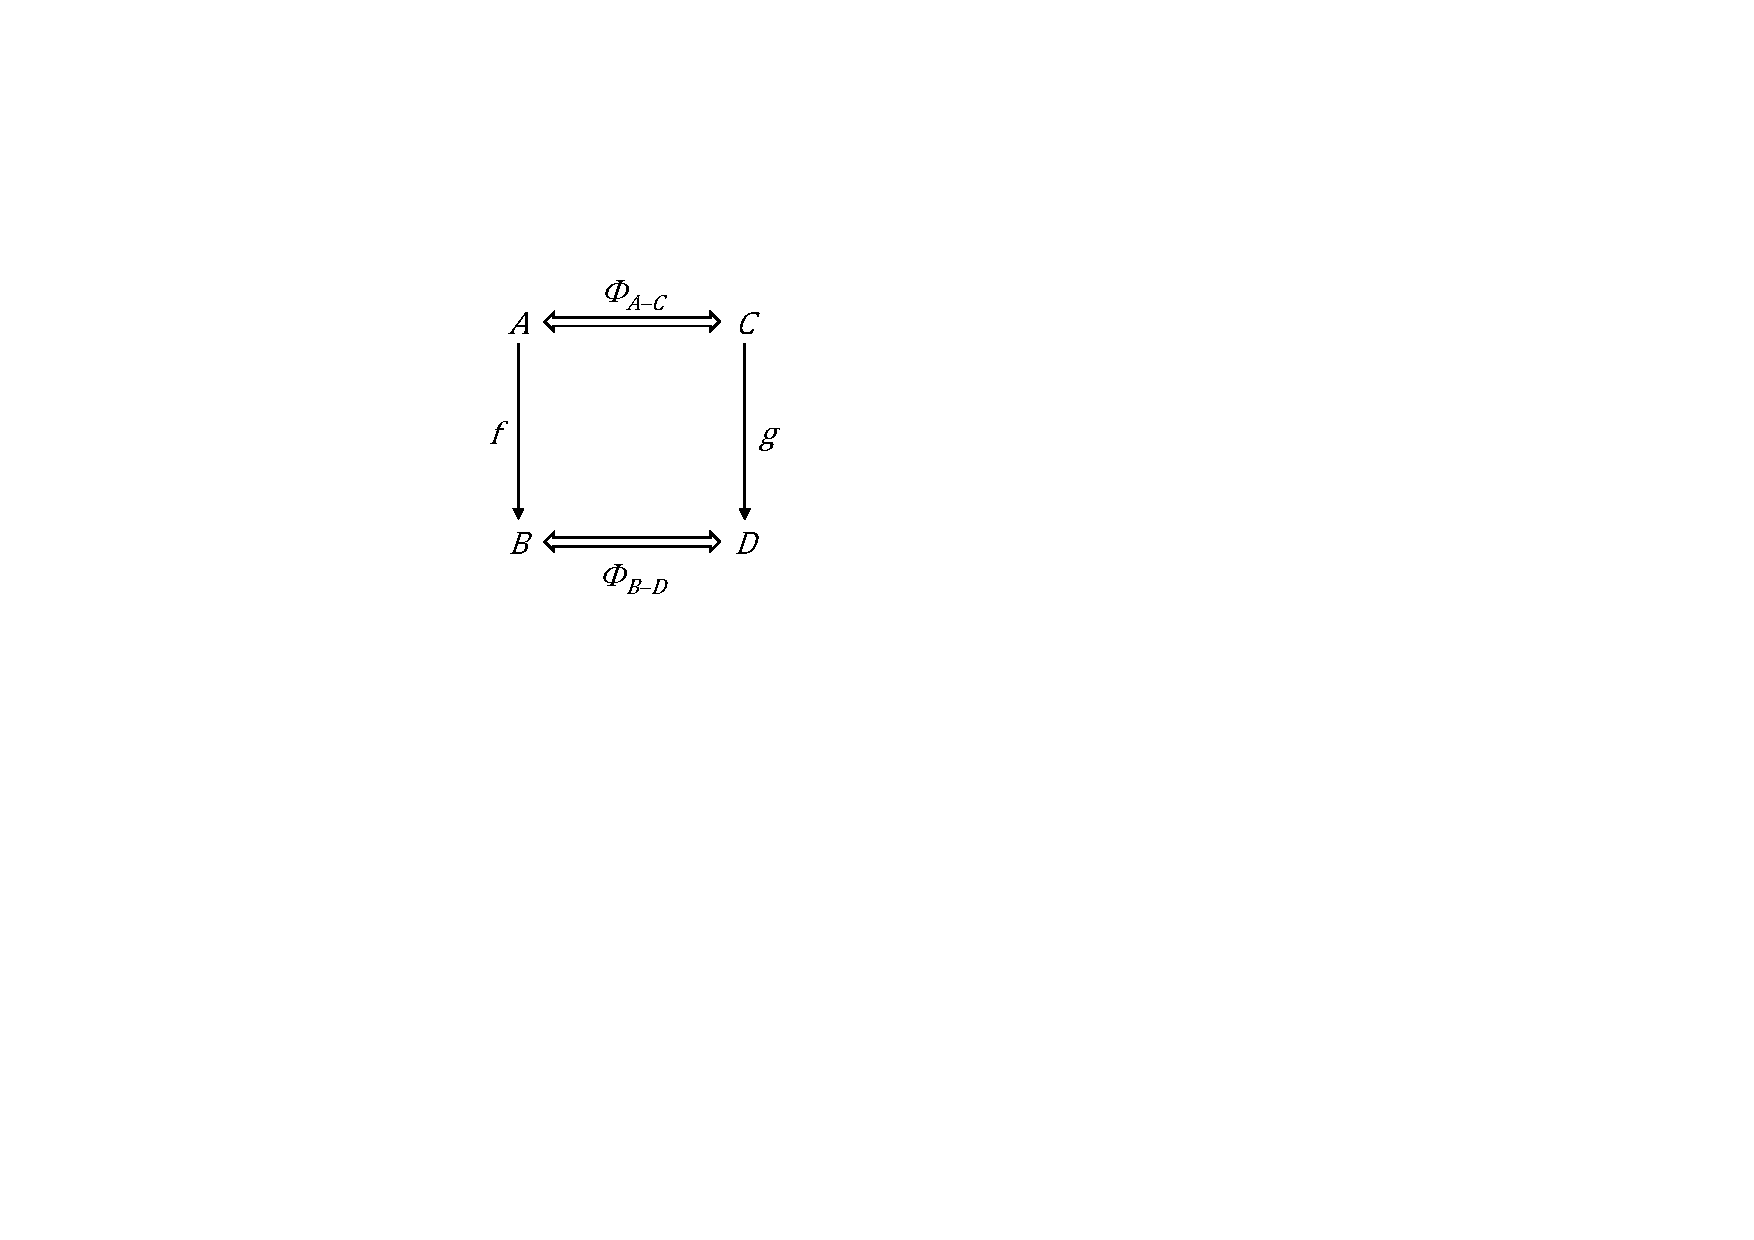
\includegraphics[width=0.35\columnwidth]{diagrams/NMFSynchronizationBlock}
	\caption{Schematic view of a synchronization block}
	\label{fig:SynchronizationBlock}
\end{figure}

The overall synchronization is specified in terms of \emph{synchronization blocks}, which are illustrated schematically in Figure~\ref{fig:SynchronizationBlock}. The isomorphisms mentioned above are represented by horizontal arrows. The isomorphism $\varPhi_{A-C}$ on the top is called \emph{base isomorphism}, while $\varPhi_{B-D}$ at the bottom plays the role of the \emph{target isomorphism}. A target isomorphism may occur as base isomorphism in another synchronization block, resulting in nested synchronization blocks. Furthermore, an isomorphism may play the role of a base isomorphism in multiple synchronization blocks, meaning that multiple consistency relations are required for making a pair of elements in the base isomorphism consistent.

The vertical arrows labeled with $f$ and $g$ denote \emph{intra-model lenses}. An intra-model lense is composed of a pair of functions called \emph{Get} and \emph{Put}. \emph{Get} and \emph{Put} are queries and updates on model elements --- in the simplest case getters and setters of element properties --- which have to satisfy round-trip laws: (1) Putting the result returned from a \emph{Get} does not change the state of the model; (2) Getting a value after a \emph{Put} returns the argument passed to the \emph{Put} operation.

Depending on the results returned from \emph{Get} operations, synchronization blocks may be classified into single-and multi-valued blocks. In the case of a \emph{single-valued block}, the \emph{Get} functions return single values which have to be consistent (e.g., the values are required to be equal). For a \emph{multi-valued block}, the \emph{Get} functions return collections. In this case, an isomorphism between these collections must be established.

The consistency relation between two models is defined by the synchronization blocks, using only the \emph{Get} operations. For consistency restoration, the \emph{Put} operations, are required, as well. For example, in a forward transformation the \emph{Get} operations on the source model are needed to retrieve the source model elements with which consistency has to be established in the target model. For updating the target model, the corresponding \emph{Put} operations are required. In simple situations, a \emph{Put} operation may be derived from the \emph{Get} operation. Otherwise, the transformation developer has to provide an explicit specification of \emph{Put} satisfying the round-trip laws of intra-model lenses. 

Altogether, the transformation developer defines the consistency relation declaratively in a functional style with the help of synchronization blocks and their \emph{Get} operations. This specification is complemented with the provision of \emph{Put} operations, which are written in a procedural style. A single specification suffices to define mutual consistency; in this regard, NMF Synchronizations is a bidirectional language. This specification is complemented with unidirectional procedural parts defining how consistency is restored in forward and backward direction, respectively.

\subsubsection{Solution}
\label{sec:solutionNMF}

NMF Synchronization is an \emph{internal DSL} based on the host language C\#. The following description is based on the solution in NMF Synchronizations submitted to TTC 2017 \cite{Hinkel2017}. Listing~\ref{lst:nmf} shows fragments of this solution, to be explained below. Since NMF Synchronization is a part of \emph{NMF} \cite{Hinkel2016}, the .NET Modeling Framework, the solution to the Families to Persons benchmark runs in a separate process which communicates with the EMF-based Benchmarx process via data streams. Below, we will not explain how this coupling is implemented; rather, we will focus on the actual core solution.



\lstdefinelanguage{cs}{
	morekeywords = {using,namespace,class,override,void,null,public,protected,private,static,out,bool,string,return,var,new,true,false,if,else,as},
	morecomment=[l]{--},
	morecomment=[s]{/*}{*/}
}


\begin{lstlisting}[label={lst:nmf}, float=*t, language=cs, caption={Solution in NMF Synchronizations}]
namespace TTC2017.FamiliesToPersons.NMF {
    public class FamiliesToPersonsSynchronization : ReflectiveSynchronization {
        public class FamilyRegisterToPersonRegister : SynchronizationRule<FamilyRegister, PersonRegister> {
            public override void DeclareSynchronization() {
                SynchronizeMany(SyncRule<MemberToMember>(),
                    fam => new FamilyMemberCollection(fam),
                    persons => persons.Persons);
            }
        }

        public class MemberToMember : SynchronizationRule<IFamilyMember, IPerson> {
            public override void DeclareSynchronization() {
                Synchronize(m => m.GetFullName(), p => p.Name);
            }
        }
        
        public class MemberToFemale : SynchronizationRule<IFamilyMember, IFemale> {
            public override void DeclareSynchronization() {
                MarkInstantiatingFor(SyncRule<MemberToMember>(), 
                    leftPredicate: m => m.MotherInverse != null || m.DaughtersInverse != null);
            }
            ...
        }
        
        private class FamilyMemberCollection : CustomCollection<IFamilyMember> {
            ...
            public override void Add(IFamilyMember item) {
                var temp = item.GetExtension<TemporaryStereotype>();
                item.AddToFamily(Register, temp.IsMale, temp.LastName);
                item.Extensions.Remove(temp);
            }
            ...
        }
        ...
    }
}
\end{lstlisting} 

In NMF Synchronizations, a transformation is defined by extending classes from a library. In Listing~\ref{lst:nmf}, the overall transformation is defined by a single top-level class (starting at line~2) containing further nested classes.

A \emph{synchronization rule} includes all synchronization blocks sharing the same base isomorphism. In the Families to Persons benchmark, each synchronization rule contains just one synchronization block. A synchronization rule is defined by subclassing the generic class \code{SynchronizationRule} (lines~3, 11, and 17). This class is equipped with two generic parameters for the types of the source and the target elements of the base isomorphism, respectively. The actual synchronization blocks are defined by overriding the method \code{Declare\-Synchron\-ization} (lines~4, 12, and 18). 

Altogether, the class starting at line~3 defines a multi-valued synchronization block with a base isomorphism between the roots of the families model and the persons model (of type \code{FamilyRegister} and \code{Person\-Register}, respectively) and a target isomorphism between family members and persons. The call to the method \code{SynchronizeMany} specifies the nested synchronization rule \code{MemberToMember}, as well as the \emph{Get} functions for retrieving the collections of family members and persons as Lambda expressions. 

\code{persons.Persons} is an \emph{invertible expression}: Since the \emph{Get} function merely collects the elements obtained via a multi-valued reference, the updates may be inferred automatically. In contrast, a \emph{custom collection} is required at the opposite end, which is implemented in the helper class \code{FamilyMemberCollection} (line~25). The implementation of the helper class has to define the path for getting the elements of the collection (traversing references to families and members sequentially), which is not shown here, and has to provide an update method for adding a family member to the collection (line~27). This \code{Add} method is required in a backward transformation to insert an already created family member at the appropriate location into the families model. To this end, a custom method \code{AddToFamily} is called (line~29) which performs this insertion depending on the configuration parameters \code{PreferExistingToNew\-Family} and \code{PreferParentToChild}. The information on the gender and the last name of the family member is retrieved from temporary stereotypes attached to the model element (line~28); these stereotypes are removed in line~30.

\code{MemberToMember} defines a single-valued synchronization block which demands that the full name of the family member be synchronized with the name of the person (i.e., the respective strings must be equal). The method \code{GetFullName} composes the full name from the first name and the last name in a straightforward way. In addition to this \emph{Get} function, we need to supply the corresponding \emph{Put} to complete the definition of the intra-model lense. To this end, a custom method \code{SetFullName} is defined which sets the full name, potentially moving the member to a different family (both methods are not shown due to the lack of space).

Finally, we need to take care of the fact that the class \code{Person} is abstract and thus cannot be instantiated in forward direction. This is achieved by two synchronization rules, one of which is shown in line~17. The rule \code{MemberToFemale} refines the rule \code{MemberToMember} by defining the type to be instantiated. Please note that the base isomorphism of the synchronization is refined to \code{IFemale} on the persons model. Furthermore, the method call in line~19 defines the predicate which has to be satisfied in order to apply this refinement (the member must be a mother or a daughter).  
